\documentclass[11pt]{article}
\usepackage{graphicx}
\usepackage{natbib}
\usepackage{rotating}
\usepackage{latexsym}
\usepackage{thumbpdf}
%\usepackage{bm}
%\usepackage{amsbsy}
\usepackage{amsmath}
\usepackage{amsthm}
\usepackage{amssymb}
\usepackage{url}
\usepackage{fancyhdr}
\usepackage{rotating}
\usepackage{alltt}


%\def\be{\begin{equation}}
%\def\en{\end{equation}}
%\def\bea{\begin{eqnarray}}
%\def\ena{\end{eqnarray}}


% some definitions 
\def\be{\begin{equation}}
\def\ee{\end{equation}}
%
\def\bea{\begin{eqnarray}}
\def\eea{\end{eqnarray}}
%
\def\ltsima{$\; \buildrel < \over \sim \;$}
\def\simlt{\lower.5ex\hbox{\ltsima}}
\def\gtsima{$\; \buildrel > \over \sim \;$}
\def\simgt{\lower.5ex\hbox{\gtsima}}
%
\def\Tobs{T_{\textrm{\mbox{\tiny{obs}}}}}
\def\Tcoh{T_{\textrm{\mbox{\tiny{coh}}}}}
%
\newcommand{\m}{\langle}
\newcommand{\M}{\rangle}
%
%%%% Stas defs
\def\en{\end{equation}}
\def\ena{\end{eqnarray}}
\newcommand {\ban} {\begin{eqnarray}} 
\newcommand {\ean} {\end{eqnarray}}
\def\di{\partial}
\def\bSo{{\bf \hat{S}_1}}
\def\bSt{{\bf \hat{S}_2}}
\def\bL{{\bf \hat{L}_{N}}}
\def\bk{{\bf \hat{k}}}
\def\bp{{\bf p} }
%%%%%%%
%
% definitions for emri's document
%%%%%%%%


\def\etal{{\it et al.}}  \def\ie{{\it i.e.}}  \def\eg{{\it e.g.}}
\def\lap{\hbox{${_{\displaystyle<}\atop^{\displaystyle\sim}}$}}
\def\gap{\hbox{${_{\displaystyle>}\atop^{\displaystyle\sim}}$}}
\def\lesssim{\mathrel{\hbox{\rlap{\hbox{\lower4pt\hbox{$\sim$}}}\hbox{$<$}}}}
\def\gtrsim{\mathrel{\hbox{\rlap{\hbox{\lower4pt\hbox{$\sim$}}}\hbox{$>$}}}}
\def\alt{\mathrel{\hbox{\rlap{\hbox{\lower4pt\hbox{$\sim$}}}\hbox{$<$}}}}
\def\agt{\mathrel{\hbox{\rlap{\hbox{\lower4pt\hbox{$\sim$}}}\hbox{$>$}}}}


%define page size
\setlength{\textheight}{9.0in}
\setlength{\textwidth}{6.5in}
\setlength{\topmargin}{-0.25in}
\setlength{\oddsidemargin}{0in}
\setlength{\evensidemargin}{0in}

%set up headers and footers on each page
%\pagestyle{fancy}
%\fancyhf{}
%\lhead{\bf\begin{tabular}{c}Section\\\thesubsection\end{tabular}}
%\chead{\bf\leftmark}
%\rhead{\bf\begin{tabular}{c}Page\\\thepage\end{tabular}}
%\lfoot{\bf\versionnumber}
%\cfoot{\bf Page~\thepage}
%\rfoot{\bf\today}



\begin{document}

\title{\bf Report on the first round of the Mock LISA Data Challenges}

\author{The \emph{Mock LISA Data Challenge Task Force}: \\ [5pt]
Keith A. Arnaud$^{(1)}$,
Stanislav Babak$^{(2)}$,
John G. Baker$^{(1)}$,
Matthew J. Benacquista$^{(3)}$, \\
Neil J. Cornish$^{(4)}$,
Curt Cutler$^{(5)}$,
Shane L. Larson$^{(6)}$,
Edward K.~Porter$^{(2)}$, \\
B. S. Sathyaprakash$^{(7)}$,
Michele Vallisneri$^{(5)}$,
Alberto Vecchio$^{(8,9)}$
Jean--Yves Vinet$^{(10)}$\\ [20pt]
\small $^{(1)}$ Gravitational Astrophysics Laboratory, NA SA Goddard Space Flight Center, \\ 
\small 8800 Greenbelt Rd., Greenbelt, MD 20771, US \\
\small $^{(2)}$ Max-Planck-Institut f\"ur Gravitationsphysik (Albert-Einstein-Institut), \\ 
\small Am M\"uhlenberg 1, D-14476 Golm bei Potsdam, Germany \\
\small $^{(3)}$ Center for Gravitational Wave Astronomy, University of Texas at Brownsville, \\ 
\small Brownsville, TX 78520, USA \\
\small $^{(4)}$ Department of Physics, Montana State University, \\
\small Bozeman, MT 59717, USA \\ 
\small $^{(5)}$ Jet Propulsion Laboratory, California Institute of Technology, \\ 
\small Pasadena, CA 91109, USA \\
\small $^{(6)}$ Department of Physics, Weber State University \\
\small 2508 University Circle, Ogden, UT 84408, USA \\ 
\small $^{(7)}$ School of Physics and Astronomy, Cardiff University, \\ 
\small Cardiff, CF243YB, UK \\
\small $^{(8)}$ School of Physics and Astronomy, University of Birmingham, \\ 
\small Edgbaston, Birmingham B152TT, UK \\
\small $^{(9)}$ Department of Physics and Astronomy, Northwestern University, \\ 
\small Evanston, IL 60208, USA \\
\small $^{(10)}$ Department ARTEMIS, Observatoire de la C\^ote d'Azur, \\ 
\small BP 429, 06304 Nice, France \\ [20pt]
}





%\author{The taskforce\\
%{\tt http://www.tapir.caltech.edu/dokuwiki/listwg1b:home}
%}

\maketitle

\begin{abstract}

The Mock Data Challenges (MLDC) have the dual purpose of fostering the development of LISA data analysis tools and capabilities, and demonstrating the technical readiness already achieved by the gravitational-wave community in distilling a rich science payoff from the LISA data output. The first round of MLDCs has just been completed: nine data sets containing simulated gravitational wave signals produced either by galactic binaries or massive black hole binaries embedded in simulated LISA instrumental noise were released in June 2006 with deadline for submission of results at the beginning of December 2006. Ten groups have participated to this first round of challenges. Here we summarise the results and provide a first critical assessment of the entries.

\end{abstract}


\section{Introduction}

At the LISA International Science Team (LIST) meeting of December 2005, the Working Group on Data Analysis (LIST-WG1B) decided to embark in the organisation of several rounds of Mock Data Challenges (MLDC), with the dual purpose of (i)  fostering the development of LISA data analysis tools and capabilities, and (ii) demonstrating the technical readiness already achieved by the gravitational-wave community in distilling a rich science payoff from the LISA data output. The LISA Mock Data Challenges were also proposed and discussed at meetings organized by the US and European LISA Project that were attended by a broad cross section of the international GW community. These challenges are meant to be blind tests, but not really contests; the greatest scientific benefit stemming from them will come from the quantitative comparison of results, analysis methods, and implementations.

A Mock LISA Data Challenge (MLDC) Task Force was constituted at the beginning of 2006 and has been working since then, to formulate challenge problems of maximum efficacy, to establish criteria for the evaluation of the analyses, to develop standard models of the LISA mission and GW sources, to provide computing tools -- LISA response simulators, source waveform generators, and a Mock Data Challenge file format -- and more generally to provide any technical support necessary to the challengers. The challenges involve the distribution of several data sets, encoded in a simple standard format, and containing combinations of realistic simulated LISA noise with the signals from one or more GW sources of parameters unknown to the challenge participants, who are asked to return the maximum amount of correct information about the sources, and to produce technical notes detailing their work. 

The release of the first round of challenge data sets was announced at the Sixth LISA International Symposium hosted by Goddard in June 2006 with deadline for submission of results on 1st December 2006 -- for organizational ease, the deadline was then moved to 4th December, 2006, 00:00 EST. John Baker (Goddard) -- a member of the Task Force not participating to the first round of MLDCs -- was appointed as MLDC1 coordinator; he has responsibility for generating the challenge data sets, receiving and posting on the web the result from the challenge participants and making the key data files available to the public soon after the submission deadline. 

The challenge data sets were posted on the MLDC website~\cite{mldcweb} a few days after the end of the LISA Symposium. They include a total of 9 data sets -- they are described on the MLDC website, the Task Force wiki~\cite{mldcwiki} and \emph{Omnibus} document for Challenge-1 \cite{omnibus} -- and Training data sets (the key files with the signal parameters are public) containing signals of similar properties to those in the challenge (``blind'') data sets. The training data sets were distributed in two flavours: noisy data sets (containing signal and noise) and noise-free data sets (where only the signal as recorded by LISA was present). The software used to generate the waveforms and data sets is public and maintained under version control, with a link from the MLDC website~\cite{mldcweb}. A summary about the MLDC1 round is also provided in the two Task Force contributions to the proceedings for the Sixth LISA Symposium~\cite{mldcproc1,mldcproc2}. 

Ten groups submitted results by the deadline of 4th December 2006. The key files of the challenge data sets were posted {\em immediately} after the deadline and the reports were also made available to the public. Since then, the Task Force has been analysing the results submitted by the participants and this document provides a preliminary report on MLDC1~\footnote{It is just over a week after the submission deadline and the report is by necessity still incomplete and should be regarded as a rapidly evolving document.}. 

The Task Force and Challenge participants will further meet for a face-to-face meeting in Potsdam on 16th December 2006, just before GWDAW11, to discuss the results of MLDC1 and the ongoing effort. At that stage the Task Force will also take the opportunity to present the second round of MLDCs (due to be released later in December 2006).

MLDC1 results (and other efforts to tackle MLDC data sets that have not yet reached the necessary maturity to produce results) will also be presented in one of the sessions at GWDAW11, including a summary presentation by the TaskForce. This will provide a forum for discussion with the wider GW data analysis community. All MLDC1 participating groups are expected to be present at GWDAW11; in fact, the LISA session (for which the MLDC have been selected as ``hot theme'') is the one that has received the larger number of abstracts of the whole meeting.

\section{Overview of submissions for Challenge 1}

Ten groups have submitted results for MLDC1 by the deadline~\footnote{The Task Force is aware of a handful of other groups who have been developing analysis algorithms to tackle the first round of MLDCs, but results were not produced in time for submission. We can therefore be moderately optimistic about having more participating groups to the second round of challenges, although they contain data sets of much more significant complexity}. Results are posted on the MLDC website~\cite{mldc-results} that includes the technical note submitted by the challenge participants and the files with the ``best parameter fits'' for the data sets. The table below provides a summary of participation to the analysis of MLDC1.

\begin{center}
\begin{tabular}{l|ccccccccc}
\hline \hline
Group              &    \multicolumn{9}{c}{Challenge identifies} \\
\hline
                   &    \multicolumn{7}{c}{Galactic binaries} & \multicolumn{2}{c}{Massive black holes} \\
                   &    \multicolumn{3}{c}{Single source} & \multicolumn{4}{c}{Multiple sources} & \multicolumn{2}{c}{Single source} \\
                   &    1.1.1a & 1.1.1b  & 1.1.1c & 1.1.2 & 1.1.3 & 1.1.4 & 1.1.5 & 1.2.1 & 1.2.2 \\

AEI             & $\bullet$  &  $\bullet$  &  $\bullet$  &  $\bullet$  &  $\bullet$  &  $\bullet$  &  $\bullet$  &  & \\
Ames              & $\bullet$  &  $\bullet$  &             &  $\bullet$  &  $\bullet$  &   &   &  & \\ 
APC              & $\bullet$  & & & & & &  \\
Goddard           & & & & & & & & $\bullet$  &  $\bullet$ \\ 
GLIG               & & & $\bullet$  & & & & & & \\
Krolak            & $\bullet$  &  $\bullet$  &  $\bullet$  &  &  $\bullet$  &    &   &  & \\ 
JPL-Caltech       & & & & & & & & $\bullet$  & \\
MT-AEI            & & & & & & & & $\bullet$  &  $\bullet$ \\ 
MT-JPL             &  $\bullet$  &    $\bullet$  &    $\bullet$  &    $\bullet$  &    $\bullet$  &    $\bullet$  &  $\bullet$  &  \\
UTB               & $\bullet$  &  $\bullet$  &  $\bullet$  &  $\bullet$  &  $\bullet$  &  $\bullet$  &  $\bullet$  &  & \\
\hline
\end{tabular} \\
\end{center}

An important point to note is that each Challenge data set, including the two data sets containing an unknown number of overlapping sources (1.1.4 and 1.1.5) was analysed by at least two groups. It is also reassuring that at this early stage of the programme several techniques are being pursued: challenge data sets were tackled with matched-filtering, Markov Chain Monte Carlo methods, Hilbert transform, tomographic reconstruction and time-frequency methods, in cases in combination to produce a multi-stage (or hierarchical) analysis approach. Matched-filtering and MCMC were applied to both galactic binaries data sets and massive black hole data sets. The vast majority of the reports emphasise that the participating groups have just begun the process of implementing these pipelines that are therefore not mature, or even at a very early stage of development. A comparison of the approaches is therefore not yet possible (or wise), but the results of the initial MLDC is reassuring on the fact that for MLDC2 a wealth of information will be available to produce a very first assessment of the different approaches.

\section{Challenge 1 results -- Galactic binaries}

A total of seven collaborations submitted entries related to galactic binaries.
Most of these entries covered the single source data sets of Challenge 1.1.1.
Several groups also had entries in the isolated source Challenges, 1.1.2
and 1.1.3, and two groups tackled the overlapping source Challenges 1.1.4 and
1.1.5.

The recovered source parameters are used to generate templates that are then
compared to the challenge data sets. For the single source challenges a comparison
was also made between the injected and recovered parameters.

The recovered templates were used to compute a number of quantities that
measure the fidelity of the parameter recovery. The first is the $\chi^2$
per degree of freedom,
\begin{equation}
\chi^2 = \frac{ ( s -h_{\rm rec} | s -h_{\rm rec})}{N -D} \, .
\end{equation}
Here $s$ denotes the challenge data, $h_{\rm rec}$ is the recovered template,
$D$ is the dimension of the model, and $N$ is the number of data points
used in computing the inner product. The noise weighted inner product, $( | )$, is
computed using the noise orthogonal pseudo $A$ and $E$ channels:
\begin{equation}
A = (2 X - Y -Z)/3, \quad \quad E = (Z-Y)/\sqrt{3} \, .
\end{equation}
For the single source data sets 200 frequency bins were used in the
inner product, so $N=800$ and $D=7$. A second quantity that was calculated
is the signal-to-noise of the recovered signal, which we define as
\begin{equation}
{\rm SNR} = \frac{(s | h_{\rm rec})}{(h_{\rm rec} | h_{\rm rec})^{1/2}} \, .
\end{equation}
The final quantity that we compute is the degree of correlation between the
noise free signal (which we generated using the key file) and the
recovered template:
\begin{equation}
C = \frac{( h_{\rm key} | h_{\rm rec})}{(h_{\rm key} | h_{\rm key})^{1/2}(h_{\rm rec} | h_{\rm rec})^{1/2}} \, .
\end{equation}

The results of applying these measures to the entries to Challenges 1.1.1a,
1.1.1b and 1.1.1c are displayed in Tables \ref{Challenge1.1.1a},
\ref{Challenge1.1.1b} and \ref{Challenge1.1.1c}. The correlation values
for the entries from Krolak and APC showed obvious signs of misphasing
of the signal. From the recovered parameter values it was clear that
the initial phase, and in some cases the polarization angles, were
out by multiples of $\pi/2$. The starred entries for Krolak and APC indicate that
the MLDC taskforce rephased the template by adding some multiple of
$\pi/2$ to the initial phase and the polarization angle (Note: this
is not the same thing as the overall degeneracy between solutions with
$\psi \rightarrow \pi/2$ and $\phi_0 \rightarrow \phi_0 - \pi$. The
recovered parameters are incorrect, and these groups should correct their
template codes for the next round).

After the re-phasing, most entrants did very well on Challenges 1.1.1a and
Challenges 1.1.1b. On the other hand, it appears that something went wrong
for most of the entrants in Challenge 1.1.1c. Challenge 1.1.1c is the
first one where the transfer functions play a significant role, and clearly
this impacted most groups. It will be interesting to hear what the various groups
uncover as the explanation of the problem.

\begin{table*}[t]
\caption{\label{Challenge1.1.1a}Challenge 1.1.1a Evaluation}
\begin{center}
\begin{tabular}{|l|c|c|c|}
\hline
Entrant  & $\chi^2$ & SNR & $C$ \\
 \hline
Key File   & 1.123382 & 51.137 &  1.000000\\
MT/JPL BAM & 1.119815 & 51.178 &  0.997979 \\
MT/JPL GA  & 1.122909 & 51.138 &  0.997668 \\
AEI        & 1.191448 & 50.604 & 0.989346 \\
Krolak     & 7.789006 & 0.933 & -0.003590 \\
Krolak*   & 1.138955 & 51.038 & 0.998855 \\
APC       & 4.830442 & -8.007 & -0.134816 \\
APC*      & 3.104782 & 50.385 & 0.989665 \\
Ames      & 1.173324 & 51.032 & 0.996947 \\
\hline  
\end{tabular}
\end{center}
\end{table*}

\begin{table*}[t]
\caption{\label{Challenge1.1.1b}Challenge 1.1.1b Evaluation}
\begin{center}
\begin{tabular}{|l|c|c|c|}
\hline
Entrant  & $\chi^2$ & SNR & $C$ \\
 \hline
Key File   & 1.011716 & 37.251 & 1.000000 \\
MT/JPL BAM & 1.049210 & 36.856 & 0.980309 \\
MT/JPL GA  & 1.053097 & 36.808 & 0.978685 \\
AEI        & 1.387298 & 33.104 & 0.874413 \\
Krolak     & 8.433994 & -37.038  & -0.995771 \\
Krolak*   & 1.039869 & 37.038  & 0.995771 \\
Ames      & 1.465105 & 32.067 & 0.822034 \\
\hline  
\end{tabular}
\end{center}
\end{table*}

\begin{table*}[t]
\caption{\label{Challenge1.1.1c}Challenge 1.1.1c Evaluation}
\begin{center}
\begin{tabular}{|l|c|c|c|}
\hline
Entrant  & $\chi^2$ & SNR & $C$ \\
 \hline
Key File   & 0.645849 & 91.579 & 1.000000 \\
MT/JPL BAM & 7.174122 & 57.250 & 0.622660 \\
MT/JPL GA  & 10.13152 & 39.348 & 0.423913 \\
AEI        & 17.41694 & -12.982 & -0.144393 \\
Krolak     & 22.26911 & -0.464 & -0.000716 \\
Krolak*   & 1.337515 & 88.630 & 0.967977 \\
GLIG      & 13.11539 & 13.093 & 0.141656 \\
\hline  
\end{tabular}
\end{center}
\end{table*}

The alert reader will notice that the UTB entries do not appear in the main analysis
tables. This is because their analysis method only returns the frequency and sky location,
which is not enough to fully specify a template. The results of the UTB entry appear
in the parameter error tables,  \ref{Challenge1.1.1a_p}, \ref{Challenge1.1.1b_p},
and \ref{Challenge1.1.1c_p}. It is interesting to note that the Ames entry for
1.1.1a locked onto a secondary sky solution, but still provided an excellent
correlation with the noise free data, $C=0.997$. It is also interesting to note
that the MT/JPL and AEI entries for Challenge 1.1.1c provide excellent fits to
the frequency and sky location of the source, despite the fact that the correlation
with the noise free data is so poor. This suggests there is some subtle phasing
issue with the waveforms that were used.

\begin{table*}[t]
\caption{\label{Challenge1.1.1a_p}Challenge 1.1.1a Parameter Errors}
\begin{center}
\begin{tabular}{|l|c|c|c|}
\hline
Entrant  & $\Delta f$ (nHz) & $\Delta \theta$ & $\Delta \phi$ \\
 \hline
MT/JPL BAM & -1.367 & -0.0148 &  -0.0083 \\
MT/JPL GA  & -1.044 & -0.0126 & -0.0027 \\
AEI        & -1.208 & -0.0179 & 0.0008   \\
Krolak     &  0.980 &  0.0283 & -0.0077 \\
APC        &  1.343 &  0.0296 & 0.0106 \\
Ames       & -1.889 & -1.1594 & 3.1270 \\
UTB        & -3.209 &  0.1426 & 0.6030 \\
\hline  
\end{tabular}
\end{center}
\end{table*}


\begin{table*}[t]
\caption{\label{Challenge1.1.1b_p}Challenge 1.1.1b Parameter Errors}
\begin{center}
\begin{tabular}{|l|c|c|c|}
\hline
Entrant  & $\Delta f$ (nHz) & $\Delta \theta$ & $\Delta \phi$ \\
 \hline
MT/JPL BAM & 0.434 & -0.0398 &  0.0030 \\
MT/JPL GA  & 0.314 & -0.0389 &  0.0035 \\
AEI        & 0.399 & -0.0494 &  0.0005 \\
Krolak     & 0.341 &  0.0366 & -0.0039 \\
Ames       & -21.098 &  -0.6064 &  0.0038 \\
UTB        & -4.299 & -0.3910 & 0.0074 \\
\hline  
\end{tabular}
\end{center}
\end{table*}


\begin{table*}[t]
\caption{\label{Challenge1.1.1c_p}Challenge 1.1.1c Parameter Errors}
\begin{center}
\begin{tabular}{|l|c|c|c|}
\hline
Entrant  & $\Delta f$ (nHz) & $\Delta \theta$ & $\Delta \phi$ \\
 \hline
MT/JPL BAM & -0.330 & 0.0084 & -0.0013 \\
MT/JPL GA  &  0.311 & 0.0134 & -0.0006 \\
AEI        & -0.405 & 0.0126 & -0.0010 \\
Krolak     & -5.210 & 0.0586 & -0.0101 \\
GLIG       &  154.850 &  0.3060 & 0.1785 \\
UTB        & 8.577 & -0.3604 & 0.0657 \\
\hline  
\end{tabular}
\end{center}
\end{table*}

The analysis of Challenges 1.1.2 and 1.1.3 is reported in Tables \ref{Challenge1.1.2} and \ref{Challenge1.1.3}.
A closer analysis of the residuals $s-h_{\rm rec}$ showed that fits were better at low frequencies and worse
at high frequencies. For example, most of the extra $\chi^2$ for the MT/JPL BAM entry for 1.1.3 comes from a
single mis-phased source with $f=4.634797644$ mHz. This problem is very similar to what was seen with the
1.1.1c entries. It turns out the the MT/JPL group used different versions of their algorithms on different
challenges: Challenges 1.1.1a, 1.1.1b, 1.1.4 and 1.1.5 were searched using the low frequency approximation
to the LISA response, while Challenges 1.1.1c, 1.1.2 and 1.1.3 were searched using the rigid adiabatic approximation.
The latter code was put together at the last minute, with only minimal testing, and it is now clear that some
bugs remain.

\begin{table*}[t]
\caption{\label{Challenge1.1.2}Challenge 1.1.2 Evaluation}
\begin{center}
\begin{tabular}{|l|c|c|c|}
\hline
Entrant  & $\chi^2$ & SNR & $C$ \\
 \hline
Key File   & 0.926374 & 529.387 & 1.000000 \\
MT/JPL BAM & 0.933907 & 523.440 & 0.988549 \\
MT/JPL GA  & 0.951525 & 505.030 & 0.953926 \\
AEI        & 1.114532 & 330.420 & 0.624990 \\
Ames       & 0.956224 & 501.713 & 0.947939 \\
\hline  
\end{tabular}
\end{center}
\end{table*}

\begin{table*}[t]
\caption{\label{Challenge1.1.3}Challenge 1.1.3 Evaluation}
\begin{center}
\begin{tabular}{|l|c|c|c|}
\hline
Entrant  & $\chi^2$ & SNR & $C$ \\
 \hline
Key File   & 0.948490 & 120.726 & 1.000000 \\
MT/JPL BAM & 0.959345 & 97.086 & 0.796300 \\
MT/JPL GA  & 0.952557 & 111.731 & 0.913632 \\
AEI        & 0.962476 & 88.3501 & 0.726209 \\
Ames       & 0.956552 & 102.179 & 0.839383 \\
\hline  
\end{tabular}
\end{center}
\end{table*}

The results for
Challenge 1.1.4 and Challenge 1.1.5 are quoted in Tables \ref{Challenge1.1.4} and
\ref{Challenge1.1.5}. A fourth column has been added to record the number of
signals recovered, $N_s$. To get a better sense of what the $\chi^2$ is telling us,
Figure \ref{res1.1.4} shows the residual strain specral density in the A channel
(scaled in units of the noise spectral density) derived from the AEI and MT/JPL
entries. The resdiual ``confusion noise'' from the MT/JPL entry is only slightly
above the instrument noise level, while the residual from the AEI entry is significantly
larger than the instrument noise level.


\begin{figure}[h]
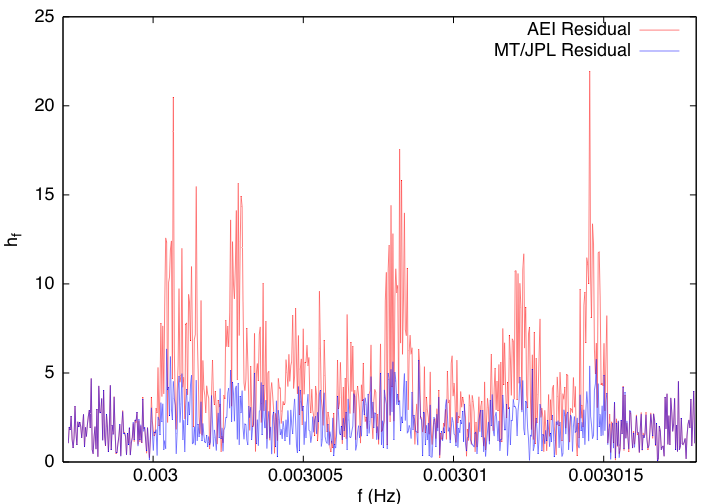
\includegraphics[angle=0,width=1.0\textwidth]{res_1_1_4.png}
\caption{\label{res1.1.4}Residual strain specral density in the A channel
(scaled in units of the noise spectral density) derived from the AEI and MT/JPL
entries.}
\end{figure}

\begin{table*}[t]
\caption{\label{Challenge1.1.4}Challenge 1.1.4 Evaluation}
\begin{center}
\begin{tabular}{|l|c|c|c|c|}
\hline
Entrant  & $\chi^2$ & SNR & $C$ & $N_s$\\
 \hline
Key File   & 1.135464 & 201.129 & 1.000000 & 45\\
MT/JPL BAM & 1.694238 & 197.827 & 0.976334 & 43\\
AEI        & 7.420979 & 159.893 & 0.791810 & 27\\
\hline  
\end{tabular}
\end{center}
\end{table*}

\begin{table*}[t]
\caption{\label{Challenge1.1.5}Challenge 1.1.5 Evaluation}
\begin{center}
\begin{tabular}{|l|c|c|c|c|}
\hline
Entrant  & $\chi^2$ & SNR & $C$ & $N_s$ \\
 \hline
Key File   &  1.299494 & 178.262 & 1.000000 & 33 \\
MT/JPL BAM &  3.276199 & 172.567 & 0.963438 & 27 \\
AEI        &  17.196080 & 116.758 & 0.654098 & 6 \\
\hline  
\end{tabular}
\end{center}
\end{table*}

\section{Challenge 1 results -- Massive black holes}

Three collaborations have submitted results for the challenge 1.2.1. Two submissions contain estimation of all nine parameters and the third one contains estimation of only chirp mass and time of coalescence.  We have only one entry for challenge 1.2.2.

In order to evaluate the results we have computed several quantities.  The noise weighted inner products were computed using the $X$-stream (used in MLDC) and two orthogonal streams with equal and uncorrelated noise:

\bea
A = (2X - Y - Z)/3; \;\;\;\; E = (Z - Y)/\sqrt{3}
\ena
and an approximate expression for the noise \bea
S = 2(S_X - S_{XY})/3
\ena
where for the frequency response used in synthetic LISA:
\bea
S_X &=& 16 \sin^2(2\pi fL)  (2 (1 + \cos^2(2\pi fL)) S_{pm} + S_{op})\\
S_{XY} &=& -4 \sin(4\pi fL)\sin(2\pi fL)  ( S_{op} + 4S_{pm} )\\
S_{pm} &=& 2.5\times10^{-48} \left(1 + \left(\frac{f}{10^{-4}Hz}\right)^{-2}
\right)  \left(\frac{f}{1Hz}\right)^{-2},\;\;\;
S_{op} = 1.8\times 10^{-37}  \left(\frac{f}{1Hz}\right)^2
\ena
We have computed the following quantities. The $\chi^2$ per degree
of freedom
\bea
\chi^{2} = \frac{(A_{data}- A_{rec}|A_{data}- A_{rec}) + 
(E_{data} - E_{rec}|E_{data} - E_{rec})}
{N-D}
\ena
and another (similar) quantity

\bea
\xi = \frac{\sqrt{(A_{data}- A_{rec}|A_{data}- A_{rec})^2 + 
(E_{data} - E_{rec}|E_{data} - E_{rec})^2}}
{N-D}
\ena
where $N$ is a number of data points and $D=9$ is number of parameters.

The next value is recovered combined SNR:
\bea
SNR  = \sqrt{SNR_A^2 + SNR_E^2},\\
SNR_A = \frac{(A_{data}|A_{rec})}{\sqrt{(A_{rec}|A_{rec})}},\;\;\;
SNR_E= \frac{(E_{data}|E_{rec})}{\sqrt{(E_{rec}|E_{rec})}}
\ena
Together with this we also compare the noiseless injected signal with 
the recovered one. Here we compute several overlaps:
\bea
O_A = \frac{(A_{key}|A_{rec})}{\sqrt{(A_{rec}|A_{rec})(A_{key}|A_{key})}}, \;\; 
O_E = \frac{(E_{key}|E_{rec})}{\sqrt{(E_{rec}|E_{rec})(E_{key}|E_{key})}}
\ena
and the overlap of the difference between the $X$ channels:
\be
O_{dX} = \frac{(X_{rec}-X_{key}|X_{rec}-X_{key})}
{\sqrt{(X_{rec}|X_{rec})(X_{key}|X_{key})}}
\en
The overlaps show how well we track the phase neglecting the error in 
the amplitude.

In order to take into account the possible error in the initial 
phase we have also computed overlaps maximized over the phase:

\bea
max_{\phi_0}(O_X) = \sqrt{(X_{rec}|X_{key}(\phi_0 = 0))^2 +
(X_{rec}|X_{key}(\phi_0 = \pi/2))^2}\\
min_{\phi_0}(O_{dX}) = \frac{ (X_{rec}|X_{rec}) + (X_{key}|X_{key}) -
2 max_{\phi_0}(X_{rec}|X_{key})}{\sqrt{(X_{rec}|X_{rec})(X_{key}|X_{key})}}
\ena

We have also computed the errors in the parameter estimations in units 
of $\sigma_{F}$, where $\sigma_{F}$ was taken from the square root of the diagonal elements of the covariance matrix (i.e. inverse of the Fisher matrix). These error estimates from the Fisher matrix were also checked against the LISA calculator.  Finally we plot the noiseless data and provide a visual comparison of the recovered signals against the key.

\subsection{Challenge 1.2.1}

We denote three entries as Montana/AEI, JPL, Goddard.
The results of computing various inner products are summarized in the 
Table~\ref{OlapsTable1.2.1}. The Montana/AEI entry has a constant phase difference (which is clear from values of
maximized overlaps), we have added one more entry (Montana/AEI*) with corrected initial phase.

\begin{table}
\caption{\label{OlapsTable1.2.1} Inner products for challenge 1.2.1}
\begin{center}
\begin{tabular}{|c|c|c|c|c|c|c|c|c|}
\hline
Entry & $\chi^2$ & $\xi$ & SNR & $O_A$ & $O_E$ & $O_{dX}$ & $min_{\phi_0}(O_{dX})$ & $max_{\phi_0}(O_X)$\\
\hline
Key & 0.5824 & 0.41182 & 667.734 &  -- & -- & -- & -- & -- \\
Montana/AEI & 0.67193 & 0.47606 & 528.023 & 0.79153 & 0.79051 &
0.41694 & 0.000128 & 0.99994\\
JPL & 0.58451 & 0.41331 & 664.471 & 0.9944 & 0.9958 & 0.0112 &  0.00909 & 0.9955\\
Montana/AEI* & 0.58331 & 0.412466 & 666.324 & 0.998 & 0.998 & 0.004 & 0.000128 & 0.99994 \\
\hline
\end{tabular}
\end{center}
\end{table}

The 9-d covariance matrix for the parameter set $\vec{x}=\{\ln(M_{c}), \ln(\mu), \ln(D_{L}), \theta_{CL}, \phi, \iota, \psi, \ln(t_{c}), \varphi_{c}\}$ evaluated with the key file is given by

\begin{tiny}
\be
\left( \begin{array}{ccccccccc}
 %3.872372e-10  &   5.487736e-09 &   -4.830902e-08 &  -6.512430e-09 &  3.874956e-09  &  -2.797328e-08  & -1.947460e-08   & 6.921398e-12  &  6.832675e-07\\
 %5.487736e-09   &  8.895662e-08  &  -4.304437e-07  &  1.219430e-08 & -6.682858e-08  &  -7.488979e-08  &  3.690754e-07   1.161215e-10   & 1.401720e-05\\
%-4.830902e-08  &  -4.304437e-07   &  3.040359e-04 &   1.676021e-05 &  7.627013e-06  &   1.280722e-04 &  -1.853579e-05  -6.568543e-12  & -1.714562e-05\\
%-6.512430e-09  &   1.219430e-08  &   1.676021e-05  &  3.293878e-06 & -2.384544e-06  &   1.123548e-05  &  1.171880e-05  -1.322383e-11  &  4.981729e-05\\
% 3.874956e-09  &  -6.682858e-08  &   7.627013e-06  & -2.384544e-06 &  4.513706e-06  &  -2.712281e-06 &  -1.819819e-05   2.635738e-11   &-7.240383e-05\\
%-2.797328e-08  &  -7.488979e-08  &   1.280722e-04  &  1.123548e-05 & -2.712281e-06  &   6.417406e-05  &  2.222767e-05   %7.460451e-12   & 1.138302e-04\\
%-1.947460e-08  &   3.690754e-07  &  -1.853579e-05  &  1.171880e-05 & -1.819819e-05  &   2.222767e-05  &  9.518923e-05   5.743921e-11   & 3.779646e-04\\
% 6.921398e-12  &   1.161215e-10  &  -6.568543e-12  & -1.322383e-11 &  2.635738e-11  &   7.460451e-12 &   5.743921e-11   1.707089e-13   & 1.785465e-08\\
% 6.832675e-07  &   1.401720e-05  &  -1.714562e-05  &  4.981729e-05 & -7.240383e-05  &   1.138302e-04  &  3.779646e-04   1.785465e-08   & 3.398534e-03
 3.87e-10  &   5.49e-09 &   -4.83e-08 &  -6.51e-09 &  3.87e-09  &  -2.8e-08  & -1.95e-08   & 6.92e-12  &  6.84e-07\\
 5.49e-09   &  8.9e-08  &  -4.30e-07  &  1.22e-08 & -6.68e-08  &  -7.49e-08  &  3.69e-07 &  1.16e-10   & 1.40e-05\\
-4.83e-08  &  -4.30e-07   &  3.04e-04 &   1.68e-05 &  7.63e-06  &   1.28e-04 &  -1.85e-05 & -6.57e-12  & -1.71e-05\\
-6.51e-09  &   1.22e-08  &   1.68e-05  &  3.29e-06 & -2.38e-06  &   1.12e-05  &  1.17e-05 & -1.32e-11  &  4.98e-05\\
 3.87e-09  &  -6.68e-08  &   7.63e-06  & -2.38e-06 &  4.51e-06  &  -2.71e-06 &  -1.82e-05 &  2.63e-11   &-7.24e-05\\
-2.8e-08  &  -7.49e-08  &   1.28e-04  &  1.12e-05 & -2.71e-06  &   6.42e-05  &  2.22e-05  & 7.46e-12   & 1.14e-04\\
-1.95e-08  &   3.69e-07  &  -1.85e-05  &  1.17e-05 & -1.82e-05  &   2.22e-05  &  9.52e-05 &  5.74e-11   & 3.78e-04\\
 6.92e-12  &   1.16e-10  &  -6.57e-12  & -1.32e-11 &  2.63e-11  &   7.46e-12 &   5.74e-11 &  1.71e-13   & 1.79e-08\\
 6.83e-07  &   1.40e-05  &  -1.71e-05  &  4.98e-05 & -7.24e-05  &   1.14e-04  &  3.78e-04 &  1.79e-08   & 3.4e-03
\end{array}
\right)
\en
\end{tiny}
%Note that off diagonal elements represented by correlation with actual parameters, not $\ln$ ({\bf Ed please confirm it}).
%This corresponds to the following values of one sigma deviation for a given in challenge 1.2.1 parameter set:
The variance-covariance matrix provides us with the following values for a 1-$\sigma$ error in the parameter estimation

\bea
M_c &=& 1.208590\times 10^6,\;\;\;     \sigma = 23.78306\\
\mu &=& 5.811961\times 10^5,\;\;\;     \sigma = 173.3452\\
D_{L} &=& 8.000000,\;\;\;     \sigma = 0.1394930\\
\theta_{CL} &=& 2.063085, \;\;\;   \sigma = 0.0018149\\
\phi &=& 0.865777 , \;\;\;      \sigma = 0.00212455\\
\iota &=& 1.94439 , \;\;\;       \sigma = 0.00801087\\
\psi &=& 3.23422, \;\;\;        \sigma = 0.0097565\\
t_{c} &=& 1.337403\times 10^7,\;\;    \sigma = 5.525738\\
\varphi_{c} &=& 4.364670, \;\;\;      \sigma = 0.058297
\ena

Note that in the above list,  the latitude has been converted to co-latitude according to $\theta_{CL}=\pi/2 - \theta_{L}$, luminosity distance and its error are quoted in Gpc, all angles are in radians, $t_{c}$ is quoted in seconds and we transform from initial orbital phase to gravitational wave phase at coalescence according to $\varphi_{c} = 2\left(\Phi_{0}-\phi(\omega(t=0))\right)$, where $\omega(t=0)$ is the orbital frequency evaluated at $t=0$.  

The errors in the parameter estimation (in units of sigma) are presented in the Table~\ref{Errors1.2.1}
\begin{table}
\caption{\label{Errors1.2.1} Errors in estimation of parameters for challenge 1.2.1. Values in brackets corresponds to the 
opposite direction on the sky.}
\begin{center}
\begin{tabular}{|c|c|c|c|c|c|c|c|c|c|}
\hline
Entry & $\Delta M_c$ & $\Delta \mu $ & $\Delta D_{L}$ & $\Delta \theta $ & $\Delta \phi $ & $\Delta \iota $ &
$\Delta \psi $ & $\Delta t_c $& $\Delta \varphi_c $ \\ 
\hline
 JPL & 37.3& 36.8 &-63.2 & 566.308 (23.75)& -1493.76  (-15.08) & 165.719 & -271.752 & -8.1 &
0.074\\
Montana/AEI & -5.0 & -3.5 & 2.4  & 0.63 & 0.63 & 2.1 & 322.0 & -0.62 &  0.076 \\
Goddard & -2203 & -- & --  & --& -- & -- & -- & -- & -1433 \\
\hline
\end{tabular}
\end{center}
\end{table}


Finally in Figure~\ref{fig1.2.1} we compare the beginning and the end of the recovered signals as compared to the signals generated using the key file. 

\begin{figure}[ht]
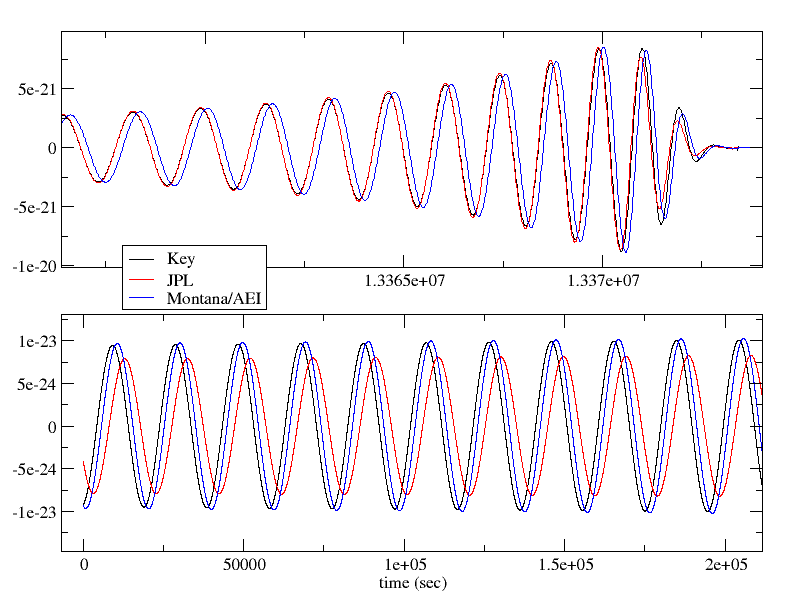
\includegraphics[angle=0,width=1.0\textwidth]{1_2_1X.png}
\caption{Comparison of the $X$-response to the signal from inspiralling SMBH. }
\label{fig1.2.1}
\end{figure}

The JPL signal provides a very good fit to the key in the LISA's most sensitive frequency band, but not across the whole bandwidth.  We can see however from Table II that even though there is a large error in the estimation of parameters for the JPL entry, the combination of these parameters results in a waveform that matches  the key-file waveform extremely well at end of the waveform where most of the SNR is accumulated.  The Montana/AEI waveform matches the amplitude and phase of the key-file signal extremely well throughout the entire bandwidth (except for the constant phase offset which has since been attributed to a missing sign allocation in the code).  When we maximize over phase we can see that the Montana/AEI overlaps truely reflect the close parameter estimation. 

 
\subsection{Challenge 1.2.2}

There is only one entry for this challenge. Here we again present the inner product and parameter estimation results, which are summarized in Table~\ref{OlapsTable1.2.2} and Table~\ref{Errors1.2.2}.  Again note that the errors for luminosity distance are given in Gpc, the error for $t_{c}$ is given in seconds and the angular errors are in radians.

\begin{table}
\caption{\label{OlapsTable1.2.2} Inner products for challenge 1.2.2}
\begin{center}
\begin{tabular}{|c|c|c|c|c|c|c|c|c|}
\hline
Entry & $\chi^2$ & $\xi$ & SNR & $O_A$ & $O_E$ & $O_{dX}$ & $min_{\phi_0}(O_{dX})$ & $max_{\phi_0}(O_X)$\\
\hline
Key & 0.58063 & 0.410566 & 106.77 & -- & -- & -- & -- & -- \\
Montana/AEI & 0.58064 & 0.41058 &  106.60 & 0.9984 & 0.9987 & 0.0033 & 0.0029 & 0.9985 \\
\hline
\end{tabular}
\end{center}
\end{table}

\begin{table}
\caption{\label{Errors1.2.2} Errors in estimation of parameters for challenge 1.2.2. }
\begin{center}
\begin{tabular}{|c|c|c|c|c|c|c|}
\hline
Entry & $\Delta M_c$ & $\Delta \mu $ & $\Delta D_{L}$ & $\Delta \theta $ & $\Delta \phi $ & $\Delta t_c $ \\ 
\hline
$\sigma_{F}$ & 97.78 & 5,273 & 8.682 & 0.00507 & 0.00527 & 2,827\\
Montana/AEI & -2.35 & -2.66 & 0.125  & 3.728 & 1.025 & -2.33  \\
\hline
\end{tabular}
\end{center}
\end{table}


The visual comparison (again beginning and end of the waveform) is presented in the figure~\ref{fig1.2.2}.  We can see in this case the phase and amplitude from the recovered signal match the key-file signal almost perfectly.

\begin{figure}[ht]
%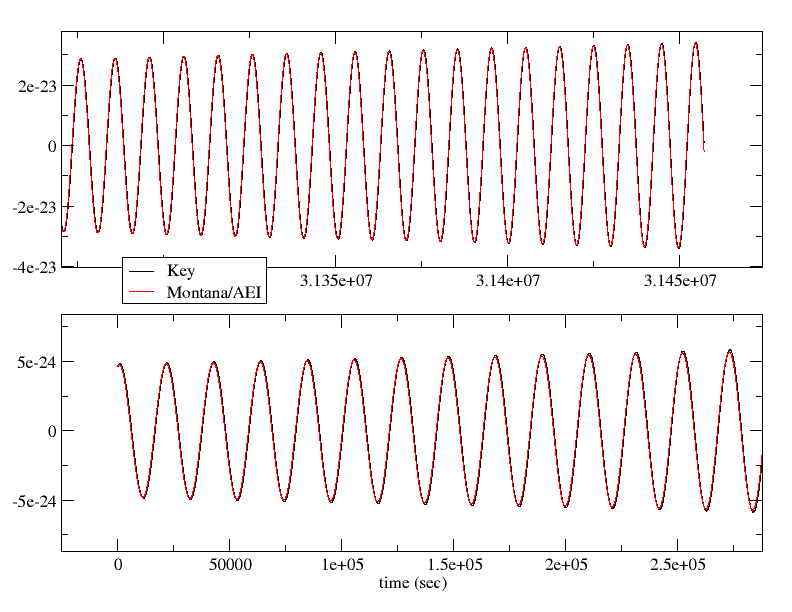
\includegraphics{Eval122.png}
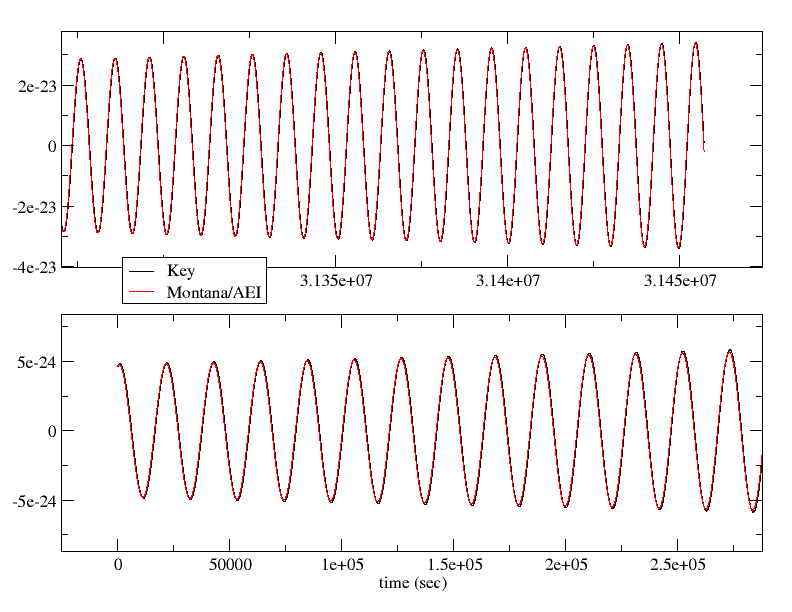
\includegraphics[angle=0,width=1.0\textwidth]{Eval122.png}
\caption{Comparison of the $X$-response to the signal from inspiralling SMBH. }
\label{fig1.2.2}
\end{figure}



\section{Conclusions}

Ten groups have submitted results to the first round of MLDCs. The Task-Force is also aware of a few other groups that have been developing analysis pipeline to tackle the MLDCs, although they have not submitted results because the algorithms are not sufficiently mature to produce even preliminary results. It is important to stress that several analysis algorithms have been developed, including matched-filter based searches, MCMCs and time-frequency methods. It is clear that only a handful of analysis pipelines have reached a sufficient degree of maturity at this stage to produce reliable results. Nonetheless, each challenge data set was tackle by more than one group, and for each challenge data set at least one entry (in several cases more than one) produced ``correct'' results, including the most challenging data set containing overlapping sources. A comparison of the performances of different algorithms is clearly premature at this stage, but these initial steps are encouraging for the outcome of MLDC2.

Several conclusion can be drawn from this first round of MLDCs: the MLDCs have made an impact on the community, and  have attracted what can be regarded as a critical mass to successfully carry out this programme; in fact, the number of entries was to some extent even larger than the Task Force had anticipated. The development work for analysis algorithms for MLDC (and LISA data analysis in general) is not concentrating in a single direction but is considering several techniques. Groups other than those traditionally engaged in LISA data analysis have entered the Challenges (in some cases with high quality results), including groups working in the analysis of ground-based data. 



\begin{thebibliography}{99}

\bibitem{mldcproc1} K.~A.~Arnaud et al. \emph{The Mock LISA Data Challenges: An overview}, gr-qc/....

\bibitem{mldcproc2} K.~A.~Arnaud et al. \emph{A Mock LISA Data Challenge How-To}, gr-qc/....

\bibitem{mldcweb} Mock LISA Data Challenge Homepage, \url{astrogravs.nasa.gov/docs/mldc}.

\bibitem{omnibus} Mock LISA Data Challenge Task Force, ``Document for Challenge 1,'' \url{svn.sourceforge.net/viewvc/lisato
ols/Docs/challenge1.pdf}.

\bibitem{mldcwiki} Mock LISA Data Challenge Task Force wiki, \url{www.tapir.caltech.edu/dokuwiki/listwg1b:home}.

\bibitem{mldc-results} \url{http://astrogravs.nasa.gov/docs/mldc/round1/entries.html}; notice that the website is still password protected (JPL still need to clear their report) but it will be made public in the next week or so (hopefully)

\end{thebibliography}

\end{document}
